\documentclass[12pt,a4paper]{article}

\usepackage[utf8]{inputenc}
\usepackage[english]{babel}
\usepackage{amsmath}
\usepackage{amsfonts}
\usepackage{amssymb}
\usepackage{graphicx}
\usepackage{lmodern}
\usepackage[left=2cm,right=2cm,top=2cm,bottom=2cm]{geometry}

\usepackage{siunitx}
\usepackage{enumitem}
\usepackage[skip=.38\baselineskip]{parskip}
\usepackage{xcolor}   % for \textcolor
\usepackage{listings}
\definecolor{mGreen}{rgb}{0,0.4,0.1}
\definecolor{mGray}{rgb}{0.5,0.5,0.5}
\definecolor{mPurple}{rgb}{0.58,0,0.82}
\definecolor{backgroundColour}{rgb}{0.95,0.95,0.92}
\lstset{
	%backgroundcolor=\color{backgroundColour},   
    commentstyle=\color{mGreen},
    keywordstyle=\color{magenta},
    numberstyle=\tiny\color{mGray},
    stringstyle=\color{mPurple},
    %breakatwhitespace=false,                        
    %captionpos=b,
    %keepspaces=true,                 
    numbers=left,                    
    numbersep=5pt,                  
    showspaces=false,                
    showstringspaces=false,
    showtabs=false,                  
    %tabsize=8,	
    language=C,    
  	basicstyle=\small\ttfamily,
  	columns=fullflexible,
  	frame=single,
  	breaklines=true,
  	postbreak=\mbox{\textcolor{red}{$\hookrightarrow$}\space},
}

% for multi-figures
\usepackage{subcaption}

\usepackage{tabularx}
\usepackage{multirow}

% for graphs
%\usepackage{tikz}
%\usepackage{tkz-graph}
%\input{tkz-graph-patch}
%\usepackage{tikz-qtree}
%\usetikzlibrary{calc, arrows, positioning}

% custom commands
\newcommand{\multilinecell}[1]{\begin{tabular}{@{}c@{}}#1\end{tabular}}

\author{Olivér Facklam}
\title{CS473: Avalon master laboratory\\Design of a camera controller}

\newcommand{\nil}{\textit{nil}}

\begin{document}
\maketitle
\tableofcontents

\section{Problem statement}

The goal of this lab is to design a camera controller which is programmable and can capture and transfer frames directly from the camera to a memory module.

The controller must expose an Avalon slave interface, allowing it to be programmed. In particular, it should have registers to set the frame buffer addresses and lengths from the processor.

The controller must also have a conduit connecting it to the camera's clock and data output. This is the interface on which the frame pixels will be sampled.

Finally, the controller must contain an Avalon master interface, enabling fast data transfer directly to memory. Ideally, this interface should support burst tranfers to speed up the flushing process.

Since the LCD display has a resolution of $320\times 240$ pixels, this is also the resolution we target for the camera frame capture. In terms of performance, we require at least 25 fps for the image to be fluid, but a frequence between 30 and 40 fps would be preferable.

\bigskip
I am working with the group composed of Samuel Thirion and Jonas Schweizer who are implementing the LCD controller.

\section{System overview}

The overall system architecture is presented in figure \ref{fig:system}. It consists of a NIOS-II processor, connected to the $I^2C$, camera and SDRAM controllers through the Avalon bus. The camera controller's master interface can also access the Avalon bus to transfer data to the memory.

The camera is connected to the FPGA through the development board's GPIO pins. The pins for serial communication are mapped to the $I^2C$ controller's \texttt{sclk} and \texttt{sdata} signals. The data signals (\texttt{data}, \texttt{fval}, \texttt{lval}) on the other hand are connected to the camera controller.

\begin{figure}[h]
	\centering
	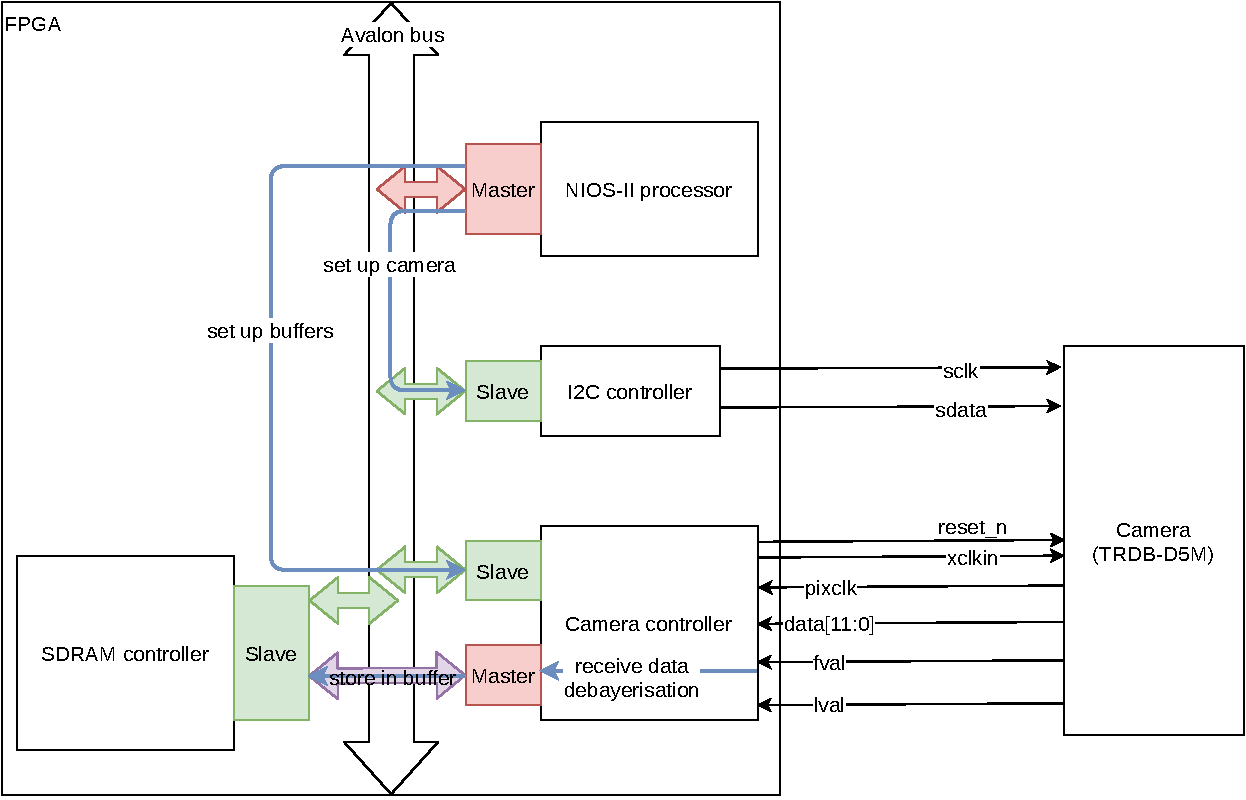
\includegraphics[width=\textwidth]{figures/system}
	\caption{Overview of system architecture and operation}
	\label{fig:system}
\end{figure}

The system typically operates according to the following high-level description:
\begin{enumerate}[nosep]
	\item The processor sets up the camera parameters by sending the appropriate commands to the $I^2C$ interface.
	\item The processor initializes some buffer regions in memory and gives the buffer information to the camera controller.
	\item The camera controller waits for the buffer to be ready.
	\item The controller captures the next whole camera frame, performing the necessary debayerisation during this process.
	\item The controller uses its master interface to copy the obtained pixel sequence to the provided buffer.
	\item The capture process can be repeated as many times as necessary, alternating between the different buffers.
\end{enumerate}

Table \ref{tab:gpio} shows how the camera pins are mapped to the system signals.

\begin{table}[ht]
	\centering
	\begin{tabular}{|c|c|c|}
		\hline
		Signal & GPIO1 signal & Board pin \\
		\hline
		\hline
		sclk & GPIO1[24] & JP7 pin 27 \\
		\hline
		sdata & GPIO1[23] & JP7 pin 26 \\
		\hline
		reset\_n & GPIO1[17] & JP7 pin 20 \\
		\hline
		xclkin & GPIO1[16] & JP7 pin 19 \\
		\hline
		pixclk & GPIO1[0] & JP7 pin 1 \\
		\hline
		fval & GPIO1[22] & JP7 pin 25 \\
		\hline
		lval & GPIO1[21] & JP7 pin 24 \\
		\hline
		data[11:0] & GPIO1[1, 3:13] & JP7 pins 2, 4..10, 13..16 \\
		\hline
	\end{tabular}
	\caption{Development board pin assignments}
	\label{tab:gpio}
\end{table}


\section{Camera controller design}

Figure \ref{fig:architecture} shows the general architecture and exposed interfaces of the camera controller design. 

\begin{figure}[h!]
	\centering
	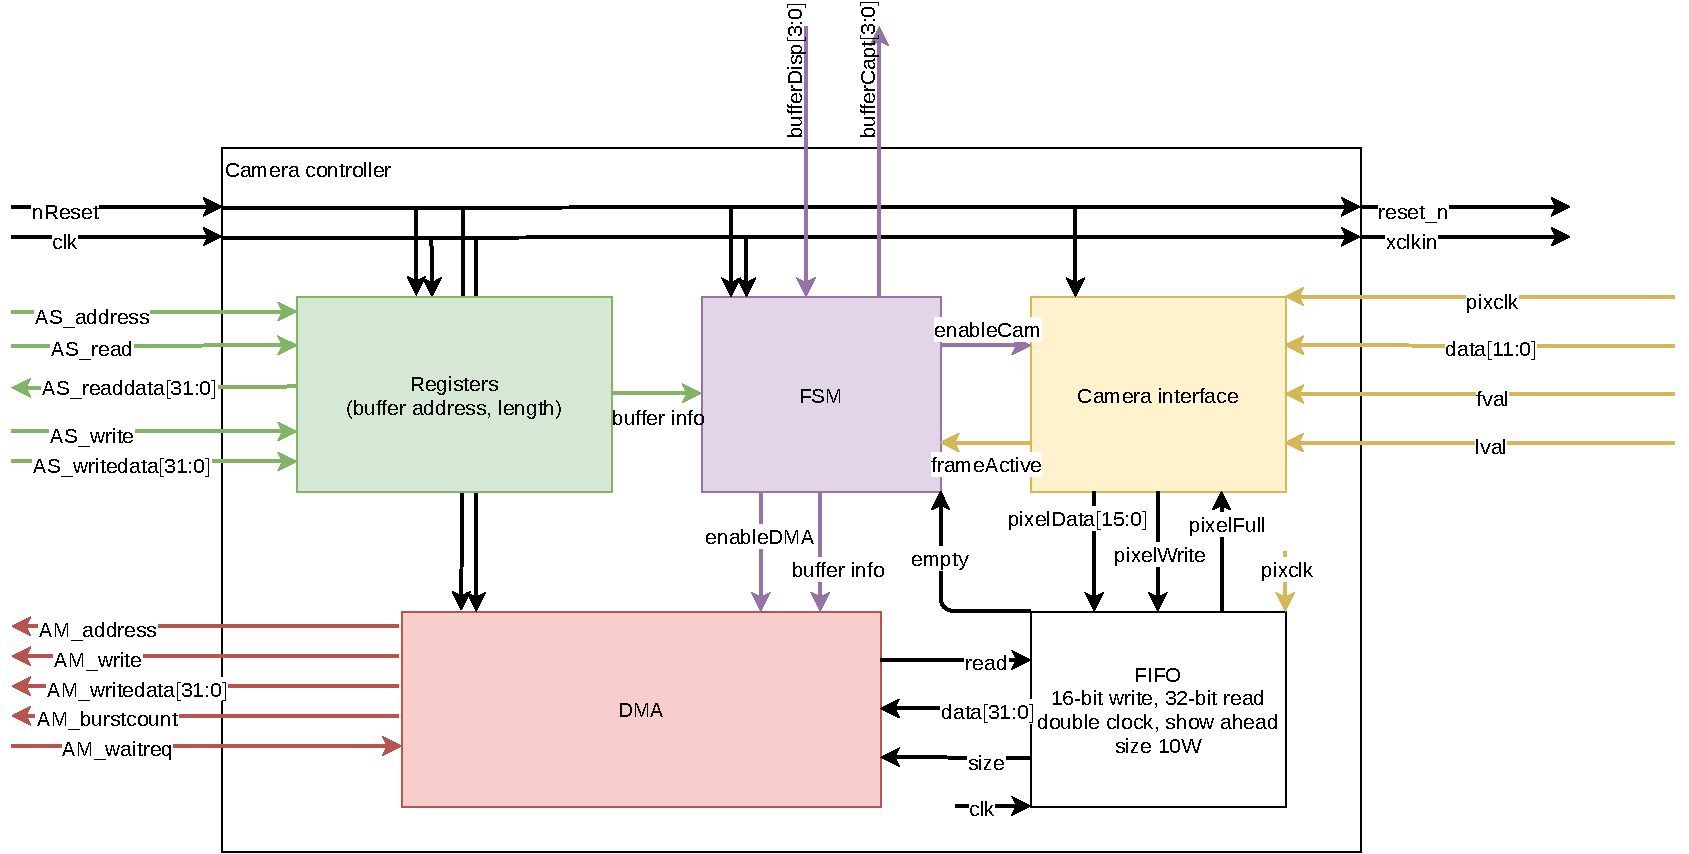
\includegraphics[width=\textwidth]{figures/architecture}
	\caption{Architecture \& signals of the camera controller}
	\label{fig:architecture}
\end{figure}


\subsection{Interfaces \& register map}

The camera controller exposes 5 different interfaces.
\begin{description}[nosep]
	\item[In black:] the \SI{50}{\mega\hertz} FPGA clock input, alongside the associated reset signal.
	\item[In yellow:] a conduit interface for camera communication. This interface contains the clock and reset input to the camera, as well as the pixel clock, data and frame/line valid signals.
	\item[In purple:] a conduit interface for synchronization. In the final system, these signals will be connected to the LCD controller to determine the states of the different buffers. The \texttt{bufferDisp} input signal denotes when a buffer is being emptied by the LCD controller; the \texttt{bufferCapt} output signal shows a buffer is being filled by the camera controller.
	\item[In green:] a 32-bit Avalon slave interface, supporting 0-wait writes and 1-wait reads. The registers accessible through this interface are described in table \ref{tab:map}.
	\item[In red:] a 32-bit Avalon master interface, supporting burst writes.
\end{description}

\begin{table}[ht]
	\centering
	\begin{tabularx}{\linewidth}{|c|c|c|X|}
		\hline
		Address & Register & Bits & Description \\
		\hline
		\hline
		0x00 & BUF0ADD & 0-31 & Address in memory of buffer 0. \\
		\hline
		\multirow{2}{*}{0x01} & BUFLEN & 0-28 & Length of each buffer. Buffer is considered valid when $\text{len} > 0$. \\
		& BUFNUMBER & 29-31 & Number of buffers. \\
		\hline
	\end{tabularx}
	\caption{Register map of the camera controller}
	\label{tab:map}
\end{table}

\subsection{Internal architecture}

The internal architecture of the camera controller is also presented on figure \ref{fig:architecture}. The system consists of 5 blocks:
\begin{itemize}
	\item the ``Registers'' block, implementing the 0-wait write / 1-wait read Avalon slave interface, storing the values of the 2 registers described previously, and providing them to the rest of the system;
	\item the FIFO block: a double-clock, show-ahead FIFO from Quartus, with a 16-bit write bus (driven by \texttt{pixclk}), and a 32-bit read bus (driven by \texttt{clk}), capable of storing 10 lines of pixels;
	\item the ``FSM'' block, implementing the finite state machine described in the next section, driving the \texttt{enableCam} and \texttt{enableDMA} signals;
	\item the ``Camera interface'' block, driven by the camera's pixel clock, sampling the incoming pixels and storing them in the FIFO;
	\item the ``DMA'' unit, using the buffer info to flush the data stored in the FIFO to the main memory, in bursts of half-lines.
\end{itemize}


\subsection{Finite state machine (FSM)}

Figure \ref{fig:syssm} shows the main finite state machine controlling the system operations. 

Each buffer's state is monitored through an instance of the state machine at the bottom of the figure, cycling through the 4 states based on the \texttt{bufferCapt} and \texttt{bufferDisp} signals of the synchronization interface.

The main state machine waits in the IDLE state for the next buffer to become available. It then enters an ARMED phase, waiting for the current camera frame to finish (so we can capture a whole frame). Both the camera interface and the DMA are then enabled until the end of the next frame. Finally, the state machine waits in the FLUSHING state until the FIFO is completely empty, before moving on to the next buffer.

\begin{figure}[p]
	\centering
	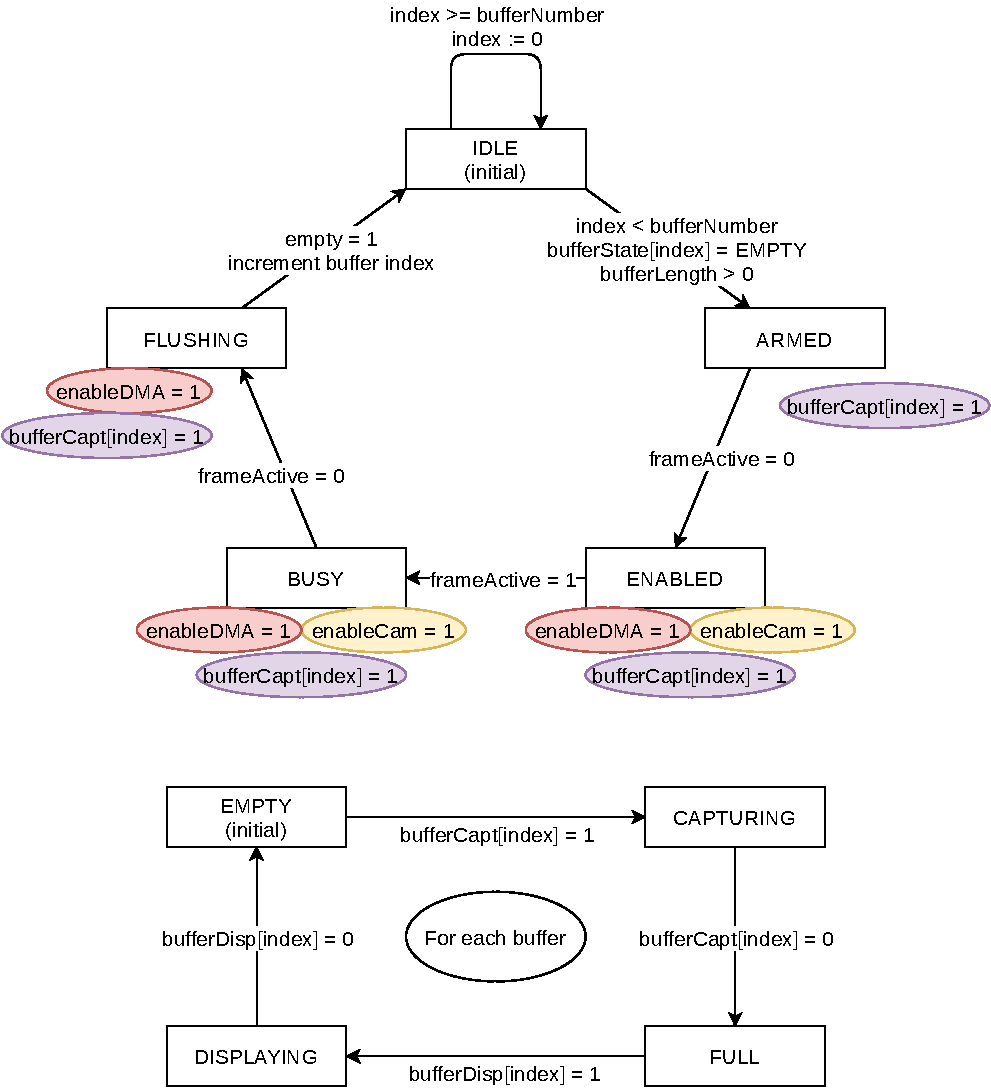
\includegraphics[width=\textwidth]{figures/syssm}
	\caption{State machine of the camera controller}
	\label{fig:syssm}
\end{figure}

\subsection{Camera interface}

The whole camera interface module is driven by the camera's pixel clock. It contains two single-clock FIFOs, respectively storing the green1 and red values. The signals and internal state machines of the camera interface are shown in figure \ref{fig:camera}.

When capturing is enabled, and the frame \& line are valid, the interface samples the incoming 12-bit data on the falling edge of the pixel clock. The pixels of even rows (starting at 0) are buffered alternatively in the 2 FIFOs (G1 \& R). The pixels of odd rows are simply stored in temporary registers (B \& G2).

In parallel to the sampling of the odd rows, the green1 and red pixels are read back from the FIFOs. This allows us to group together the four colors from a $2\times 2$ square, and merge them into a single 16-bit RGB pixel. This pixel value is then output through the \texttt{pixelData} signal, and written in the main FIFO.

The state machines shown in figure \ref{fig:camera} simply keep track of the row and column parity. All the read and write signals are directly driven by some combinational logic of the input and state signals mentioned previously. These functions can be seen at the very bottom of the figure.

Typical timings for the capture of a single camera frame are shown in the diagram of figure \ref{fig:camtime}.

\begin{figure}[ht]
	\centering
	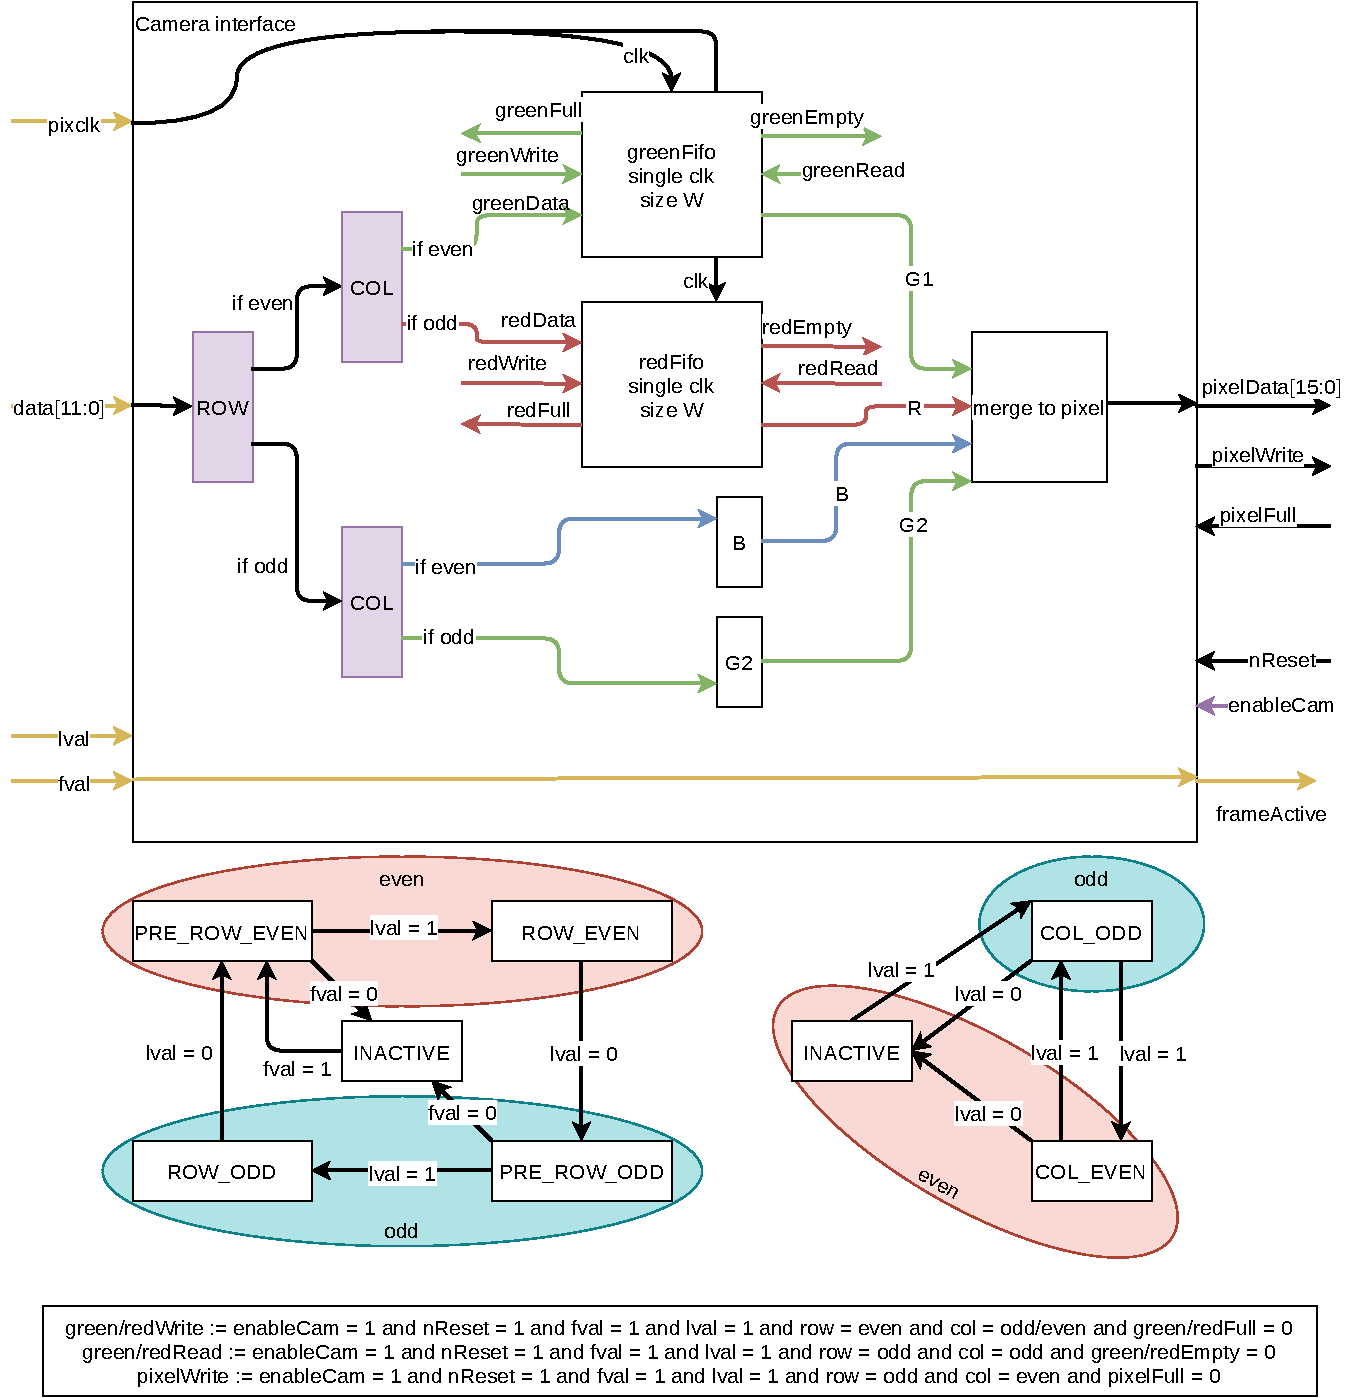
\includegraphics[width=\textwidth]{figures/camera}
	\caption{Design and operation of the camera interface block}
	\label{fig:camera}
\end{figure}

\begin{figure}[p]
	\centering
	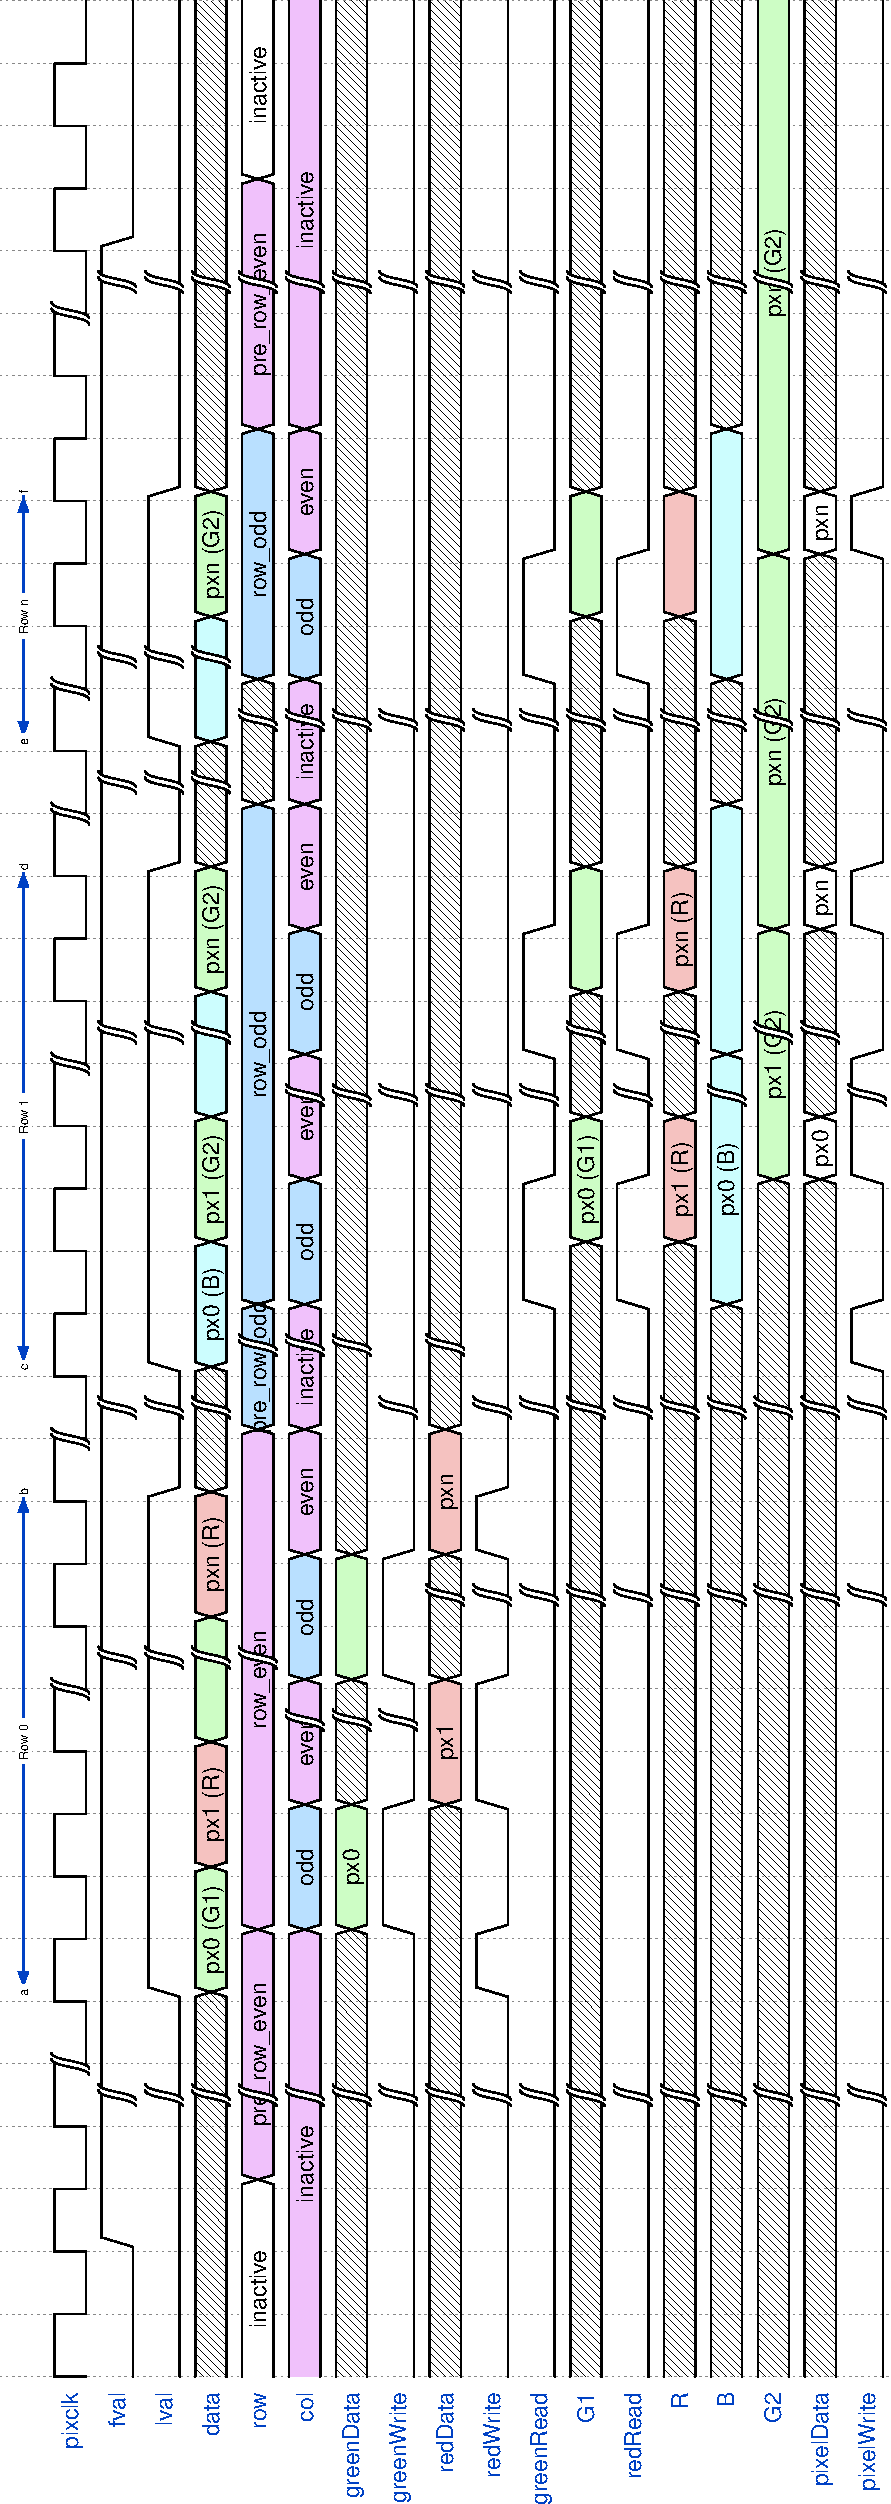
\includegraphics[width=.51\textwidth]{figures/camera_timings_rot}
	\caption{Timing of the camera interface signals during a frame capture}
	\label{fig:camtime}
\end{figure}

\newpage
\subsection{DMA unit}

The DMA unit is responsible for driving the Avalon master interface, and writing the pixels into the appriopriate memory buffer. Once enabled, the DMA keeps track of the current address we are writing to, starting from the buffer address and incrementing after every burst. The writing is done in half-line bursts (160 pixels = 80 words). At the beginning of each burst, the DMA waits in the BURSTPREPARE state, for enough pixels to become available in the FIFO. It then outputs the 80 words successively (monitoring the \texttt{AM\_waitreq} signal), keeping track with a counter. Once all pixels have been written, the burst is terminated.

The design of the DMA unit is shown in figure \ref{fig:dma}, the timing diagram in figure \ref{fig:dmatime}.

\begin{figure}[h]
	\centering
	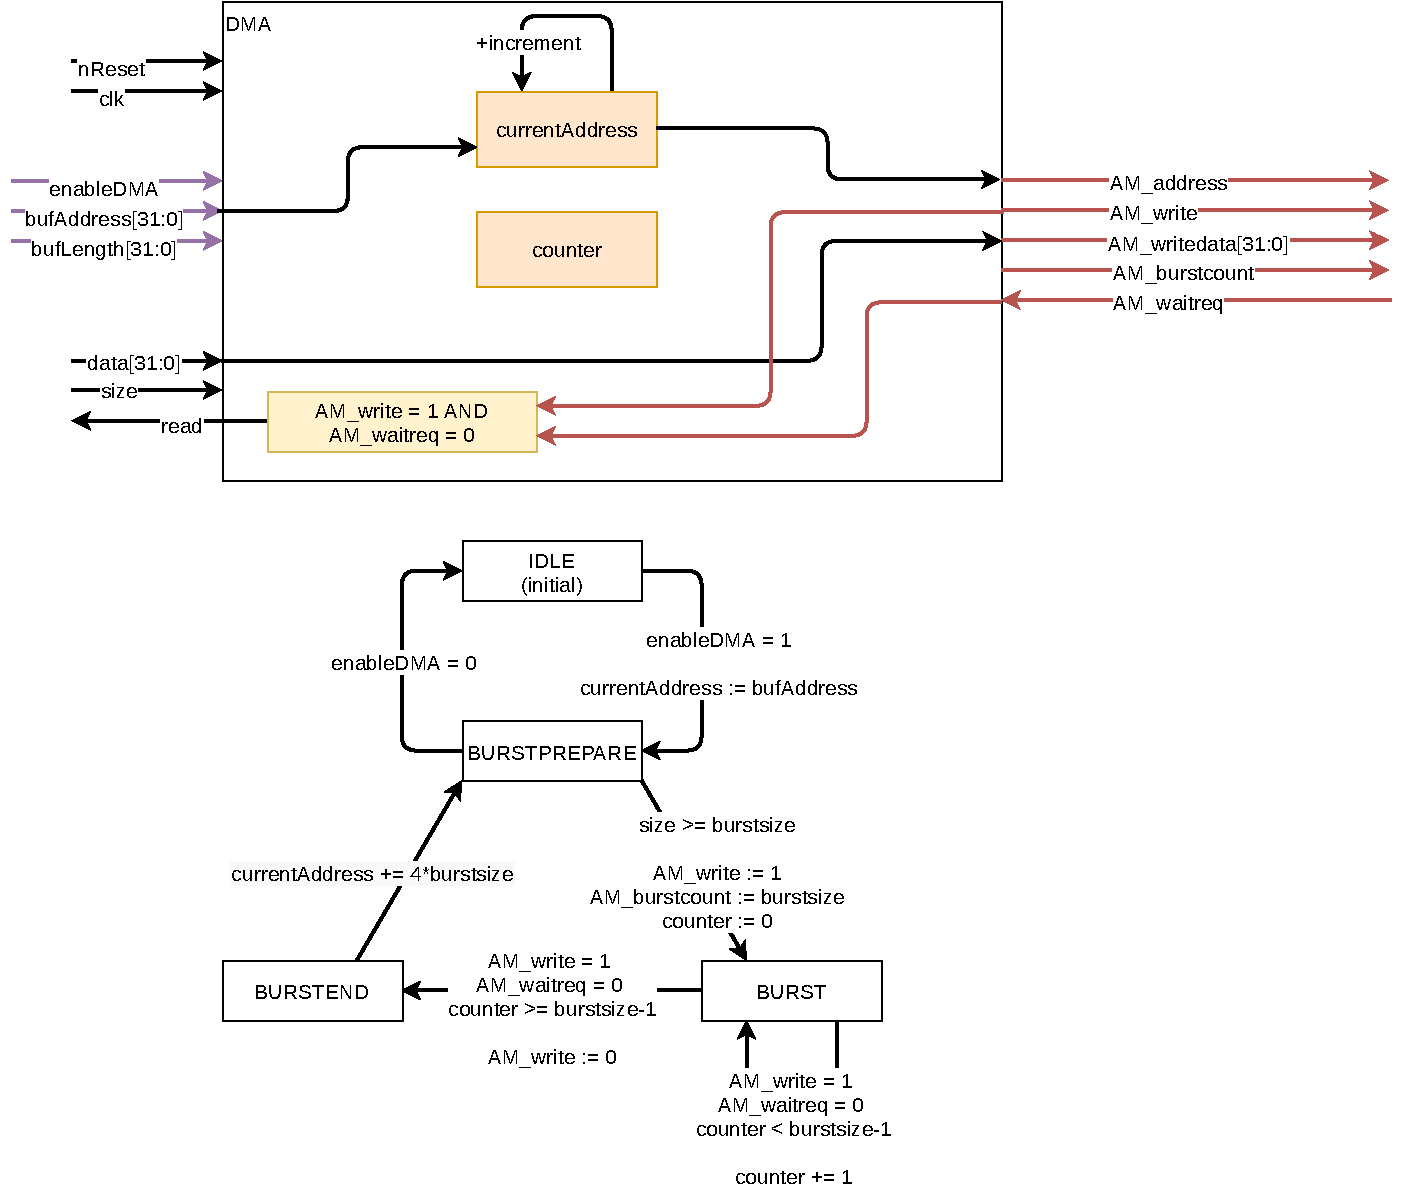
\includegraphics[width=.85\textwidth]{figures/dma}
	\caption{Design and operation of the DMA unit}
	\label{fig:dma}
\end{figure}

\begin{figure}[ht!]
	\centering
	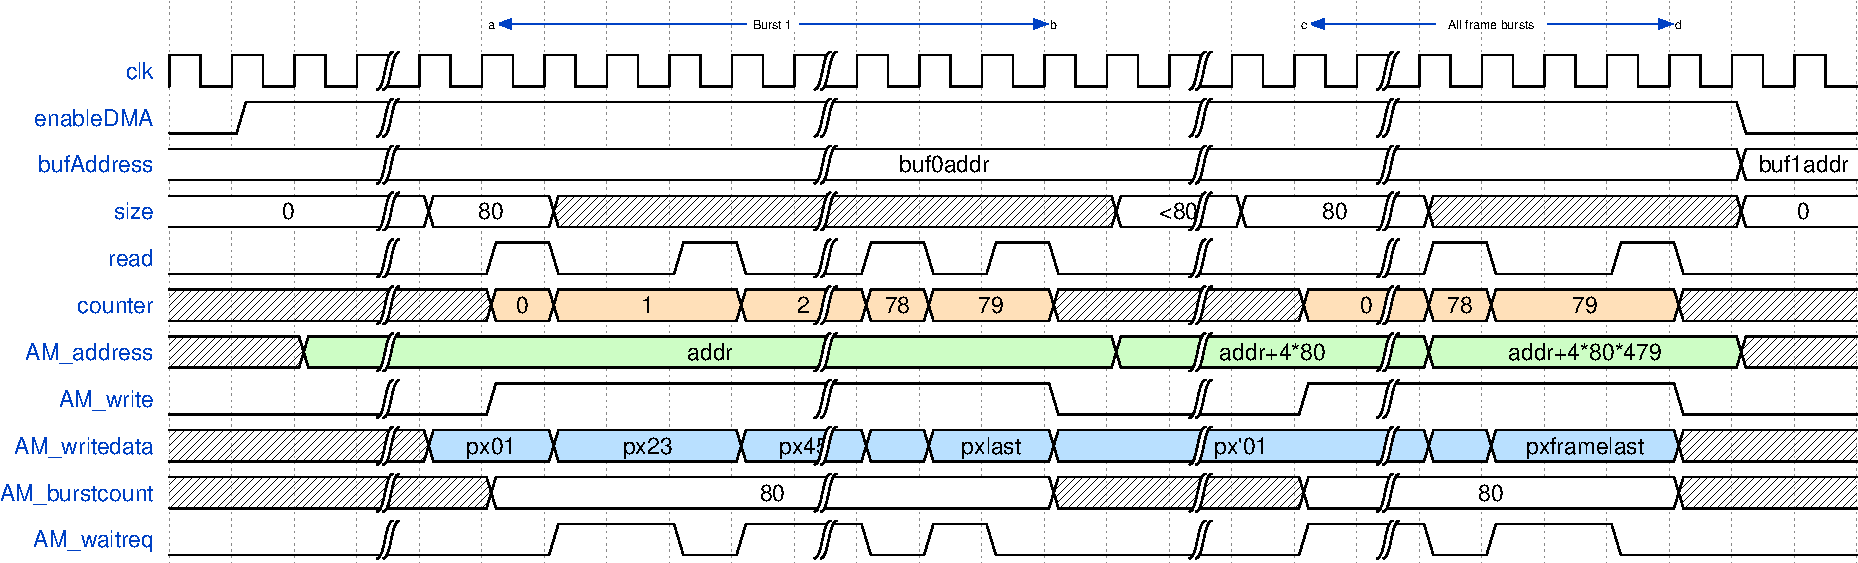
\includegraphics[width=\textwidth]{figures/dma_timings}
	\caption{Timing of the DMA signals during a frame flush}
	\label{fig:dmatime}
\end{figure}


\section{Frame buffer organization}

Pixels are stored on 16 bits in 5-6-5 RGB format, like shown in table \ref{tab:pixel}. Thus 2 pixels fit into a 32-bit word in memory.

\begin{table}[h]
	\centering
	\begin{tabular}{|c|c|c|c|c||c|c|c|c|c|c||c|c|c|c|c|}
		\hline
		15 & 14 & 13 & 12 & 11 & 10 & 9 & 8 & 7 & 6 & 5 & 4 & 3 & 2 & 1 & 0 \\
		\hline
		R4 & R3 & R2 & R1 & R0 & G5 & G4 & G3 & G2 & G1 & G0 & B4 & B3 & B2 & B1 & B0 \\
		\hline	
	\end{tabular}
	\caption{Pixel organization}
	\label{tab:pixel}
\end{table}

In the frame buffer, the 320 pixels from a camera row are stored contiguously, on 160 successive words. The 240 rows are also stored contiguously. The memory organization is shown figure \ref{fig:buffer}.

\begin{figure}[h]
	\centering
	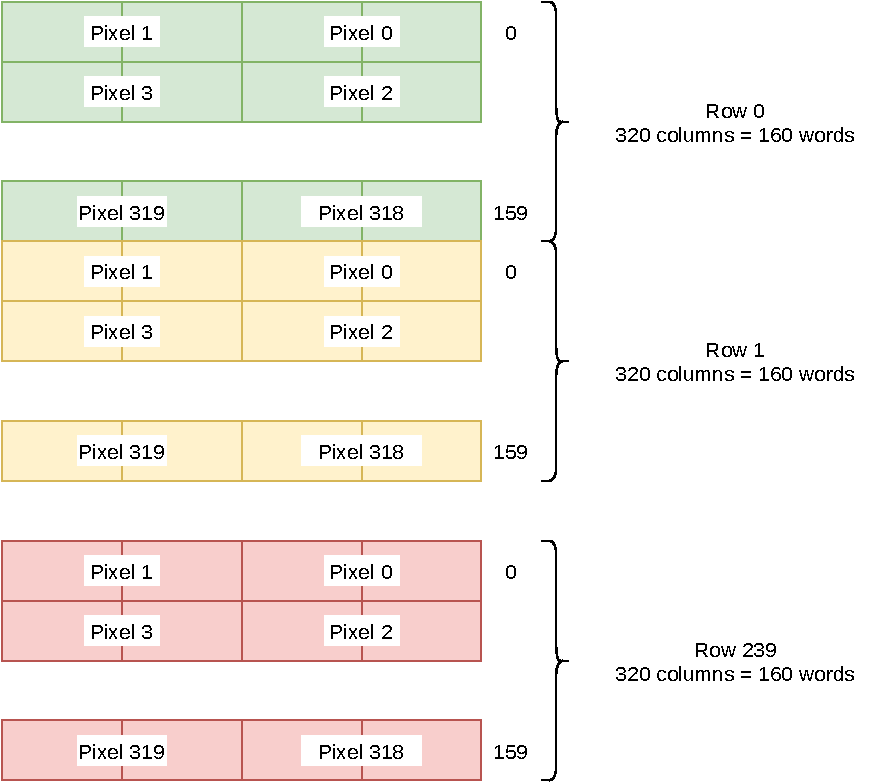
\includegraphics[width=.7\textwidth]{figures/buffer}
	\caption{Buffer organization}
	\label{fig:buffer}
\end{figure}


\section{System configuration \& operation}

During system setup, the processor must configure some important camera settings to make it work in the appropriate mode. First, the size of the captured image should be set by writing \texttt{Column\_Size} = 2559 and \texttt{Row\_Size} = 1919. Then, both row and column skip and bin should be set to 3, in order to achieve the desired resolution of $640 \times 480$. Since the camera pixels are grouped by the camera interface into $2 \times 2$ squares to form RGB pixels, this is ideal in order to create the $320 \times 240$ image we are targeting.

After the camera setup, the processor must allocate some buffer areas in the main memory, and set their information in the camera controller's registers.

From then on, the camera controller operates independently, synchronizing through the previously described conduit with the LCD controller to determine the state of the buffers and to rotate them.



\end{document}